\documentclass[a4paper, 10pt]{article}
\usepackage{scrextend}
\changefontsizes{9pt}
% Per-subject config for this repo. See vendor/template/course-config.tex.example
% for what each macro is used for.

\newcommand{\CourseCode}{2110515}
\newcommand{\CourseName}{Intro to Quantum Computing}
\newcommand{\StudentID}{6733172621}
\newcommand{\StudentName}{Patthadon Phengpinij}
\newcommand{\DefaultCollaborators}{Claude (for\,\LaTeX\,styling and grammar checking)}
\newcommand{\AssignmentLabel}{Assignment}

\usepackage{../vendor/template/CEDT-Assignment-style}

\begin{document}
\subject
\asgntitle{7}{}{Week 7}{\StudentID\ \StudentName}{\DefaultCollaborators}

% ================================================================================ %
%                                    Problem 01                                    %
% ================================================================================ %
\begin{problem}
\textbf{Z-Gate}
\par Use hand calculation and co-lab to show that the Z-gate converts \( \ket{-} \) to \( \ket{+} \).
\end{problem}

\begin{solution}
	\noindent \textbf{Hand calculation.} The Z-gate is \( Z = \sigma_z = \begin{pmatrix} 1 & 0 \\ 0 & -1 \end{pmatrix} \): it leaves \( \ket{0} \) alone and flips the sign of \( \ket{1} \).
	With \( \ket{-} = \tfrac{1}{\sqrt{2}}\paren{\ket{0} - \ket{1}} \),
	\[
		Z\ket{-}
		= \frac{1}{\sqrt{2}}\begin{pmatrix} 1 & 0 \\ 0 & -1 \end{pmatrix}\begin{pmatrix} 1 \\ -1 \end{pmatrix}
		= \frac{1}{\sqrt{2}}\begin{pmatrix} 1 \\ 1 \end{pmatrix}
		= \ket{+}.
	\]
	In Dirac notation the same step reads
	\[
		Z\ket{-}
		= \tfrac{1}{\sqrt{2}}\paren{Z\ket{0} - Z\ket{1}}
		= \tfrac{1}{\sqrt{2}}\paren{\ket{0} - (-\ket{1})}
		= \tfrac{1}{\sqrt{2}}\paren{\ket{0} + \ket{1}}
		= \ket{+}.
	\]
	By the same token \( Z\ket{+} = \ket{-} \): in the \( \ket{+}/\ket{-} \) basis the Z-gate acts as a NOT gate, which is the key to \textbf{Problem 2}.

	\noindent \textbf{Colab.}
	\begin{codingbox*}
Z     = np.array([[1, 0], [0, -1]])
plus  = np.array([1,  1]) / np.sqrt(2)
minus = np.array([1, -1]) / np.sqrt(2)

print(Z @ minus)
print(np.allclose(Z @ minus, plus), np.allclose(Z @ plus, minus))
\end{codingbox*}
	\noindent The notebook (\textbf{Appendix~1}) gives \( Z\ket{-} = (0.7071,\, 0.7071)^{\top} = \ket{+} \) and \texttt{True} for both checks, confirming the hand calculation.
\end{solution}
% ================================================================================ %

% ================================================================================ %
%                                    Problem 02                                    %
% ================================================================================ %
\begin{problem}
\textbf{Controlled-Z Gate}
\par Construct a controlled-Z gate from the controlled phase shift gate.
Then show that it is a CNOT gate in the \( \ket{+}/\ket{-} \) basis.
\end{problem}

\begin{solution}
	\noindent \textbf{Controlled phase shift.} The phase shift gate \( P(\varphi) = \begin{pmatrix} 1 & 0 \\ 0 & e^{i\varphi} \end{pmatrix} \) multiplies \( \ket{1} \) by \( e^{i\varphi} \).
	Its controlled version applies \( P(\varphi) \) to the target only when the control (MSB) is \( \ket{1} \):
	\[
		CP(\varphi)
		= \ket{0}\bra{0} \otimes I + \ket{1}\bra{1} \otimes P(\varphi)
		= \begin{pmatrix}
			1 & 0 & 0 & 0            \\
			0 & 1 & 0 & 0            \\
			0 & 0 & 1 & 0            \\
			0 & 0 & 0 & e^{i\varphi}
		\end{pmatrix}.
	\]

	\noindent \textbf{Controlled-Z.} Choose \( \varphi = \pi \). Since \( e^{i\pi} = -1 \), the phase shift becomes \( P(\pi) = \mathrm{diag}(1, -1) = Z \), and
	\[
		CZ = CP(\pi)
		= \ket{0}\bra{0} \otimes I + \ket{1}\bra{1} \otimes Z
		= \begin{pmatrix}
			1 & 0 & 0 & 0  \\
			0 & 1 & 0 & 0  \\
			0 & 0 & 1 & 0  \\
			0 & 0 & 0 & -1
		\end{pmatrix}.
	\]
	Only \( \ket{11} \) picks up a sign. Because that sign needs \emph{both} qubits to be \( 1 \), CZ is symmetric: it does not matter which qubit is called the control.

	\noindent \textbf{CNOT in the \( \ket{+}/\ket{-} \) basis.} Keep the control in the \( \ket{0}/\ket{1} \) basis and write the target in the \( \ket{+}/\ket{-} \) basis.
	When the control is \( \ket{0} \) nothing happens; when it is \( \ket{1} \) the target gets \( Z \), which exchanges \( \ket{+} \leftrightarrow \ket{-} \) (\textbf{Problem 1}):
	\begin{center}
		\begin{tabular}{ccc}
			\toprule
			CZ, target in \( \ket{+}/\ket{-} \)         & \qquad & CNOT, target in \( \ket{0}/\ket{1} \)       \\
			\midrule
			\( \ket{0}\ket{+} \mapsto \ket{0}\ket{+} \) &        & \( \ket{0}\ket{0} \mapsto \ket{0}\ket{0} \) \\
			\( \ket{0}\ket{-} \mapsto \ket{0}\ket{-} \) &        & \( \ket{0}\ket{1} \mapsto \ket{0}\ket{1} \) \\
			\( \ket{1}\ket{+} \mapsto \ket{1}\ket{-} \) &        & \( \ket{1}\ket{0} \mapsto \ket{1}\ket{1} \) \\
			\( \ket{1}\ket{-} \mapsto \ket{1}\ket{+} \) &        & \( \ket{1}\ket{1} \mapsto \ket{1}\ket{0} \) \\
			\bottomrule
		\end{tabular}
	\end{center}
	The two tables are the same once \( \ket{+} \) is read as ``0'' and \( \ket{-} \) as ``1'': the target flips exactly when the control is \( 1 \).

	\noindent \textbf{As a matrix.} The new basis \( \{\ket{0+}, \ket{0-}, \ket{1+}, \ket{1-}\} \) is obtained from the old one by \( I \otimes H \) (since \( H\ket{0} = \ket{+} \) and \( H\ket{1} = \ket{-} \)), and \( H = H^{\dagger} = H^{-1} \).
	So the matrix of CZ in the new basis is
	\begin{align*}
		\paren{I \otimes H}\, CZ \,\paren{I \otimes H}
		 & = \ket{0}\bra{0} \otimes HIH + \ket{1}\bra{1} \otimes HZH \\
		 & = \ket{0}\bra{0} \otimes I + \ket{1}\bra{1} \otimes X
		= \begin{pmatrix}
			  1 & 0 & 0 & 0 \\
			  0 & 1 & 0 & 0 \\
			  0 & 0 & 0 & 1 \\
			  0 & 0 & 1 & 0
		  \end{pmatrix}
		= \mathrm{CNOT},
	\end{align*}
	using \( HIH = H^2 = I \) and
	\[
		HZH
		= \frac{1}{2}\begin{pmatrix} 1 & 1 \\ 1 & -1 \end{pmatrix}\begin{pmatrix} 1 & 0 \\ 0 & -1 \end{pmatrix}\begin{pmatrix} 1 & 1 \\ 1 & -1 \end{pmatrix}
		= \frac{1}{2}\begin{pmatrix} 1 & -1 \\ 1 & 1 \end{pmatrix}\begin{pmatrix} 1 & 1 \\ 1 & -1 \end{pmatrix}
		= \frac{1}{2}\begin{pmatrix} 0 & 2 \\ 2 & 0 \end{pmatrix}
		= X .
	\]
	Hence CZ is a CNOT gate in the \( \ket{+}/\ket{-} \) basis. \( \blacksquare \)
	The notebook (\textbf{Appendix~1}) confirms \( CP(\pi) = \mathrm{diag}(1,1,1,-1) \), \( \paren{I \otimes H}\, CZ \,\paren{I \otimes H} = \mathrm{CNOT} \), and \( CZ\ket{1+} = \ket{1-} \).
\end{solution}
% ================================================================================ %

% ================================================================================ %
%                                    Problem 03                                    %
% ================================================================================ %
\begin{problem}
\textbf{Implementation of a SWAP gate}
\par A SWAP gate can be implemented using 3 CNOT gates in sequence. We will discuss this later.
But try it now to challenge yourselves.
The first and the third CNOT gates have the first bit as the control bit,
but the second CNOT gate has the second qubit as the control bit.
Try to create the matrix of the second CNOT gate and then prove the circuit is indeed a SWAP gate.
\end{problem}

\begin{solution}
	\noindent \textbf{Conventions.} Write two-qubit states as \( \ket{a\,b} \), with \( a \) the first bit (MSB) and \( b \) the second (LSB), in the order \( \ket{00}, \ket{01}, \ket{10}, \ket{11} \).
	Call the CNOT with the first bit as control \( C_M \) and the one with the second bit as control \( C_L \):
	\[
		C_M : \ket{a\,b} \mapsto \ket{a,\; a \oplus b},
		\qquad
		C_L : \ket{a\,b} \mapsto \ket{a \oplus b,\; b}.
	\]

	\noindent \textbf{Matrix of the second CNOT.} The \( j \)-th column of a gate's matrix is the image of the \( j \)-th basis state.
	For \( C_L \) the control is the LSB, so only \( \ket{01} \) and \( \ket{11} \) get their MSB flipped:
	\[
		C_L\ket{00} = \ket{00}, \quad
		C_L\ket{01} = \ket{11}, \quad
		C_L\ket{10} = \ket{10}, \quad
		C_L\ket{11} = \ket{01}.
	\]
	Placing these images as columns, and comparing with the first-bit-controlled CNOT,
	\[
		C_L = \begin{pmatrix}
			1 & 0 & 0 & 0 \\
			0 & 0 & 0 & 1 \\
			0 & 0 & 1 & 0 \\
			0 & 1 & 0 & 0
		\end{pmatrix},
		\qquad
		C_M = \begin{pmatrix}
			1 & 0 & 0 & 0 \\
			0 & 1 & 0 & 0 \\
			0 & 0 & 0 & 1 \\
			0 & 0 & 1 & 0
		\end{pmatrix}.
	\]
	So \( C_L \) exchanges \( \ket{01} \leftrightarrow \ket{11} \), while \( C_M \) exchanges \( \ket{10} \leftrightarrow \ket{11} \).

	\noindent \textbf{The circuit is a SWAP.} The gates act in the order \( C_M \), \( C_L \), \( C_M \), so the circuit's matrix is the product with the first gate on the right, \( U = C_M C_L C_M \).
	The first two gates give
	\[
		C_L C_M
		= \begin{pmatrix}
			1 & 0 & 0 & 0 \\ 0 & 0 & 0 & 1 \\ 0 & 0 & 1 & 0 \\ 0 & 1 & 0 & 0
		\end{pmatrix}
		\begin{pmatrix}
			1 & 0 & 0 & 0 \\ 0 & 1 & 0 & 0 \\ 0 & 0 & 0 & 1 \\ 0 & 0 & 1 & 0
		\end{pmatrix}
		= \begin{pmatrix}
			1 & 0 & 0 & 0 \\ 0 & 0 & 1 & 0 \\ 0 & 0 & 0 & 1 \\ 0 & 1 & 0 & 0
		\end{pmatrix},
	\]
	and the third \( C_M \), multiplied on the left, exchanges rows 3 and 4:
	\[
		U = C_M \paren{C_L C_M}
		= \begin{pmatrix}
			1 & 0 & 0 & 0 \\ 0 & 1 & 0 & 0 \\ 0 & 0 & 0 & 1 \\ 0 & 0 & 1 & 0
		\end{pmatrix}
		\begin{pmatrix}
			1 & 0 & 0 & 0 \\ 0 & 0 & 1 & 0 \\ 0 & 0 & 0 & 1 \\ 0 & 1 & 0 & 0
		\end{pmatrix}
		= \begin{pmatrix}
			1 & 0 & 0 & 0 \\ 0 & 0 & 1 & 0 \\ 0 & 1 & 0 & 0 \\ 0 & 0 & 0 & 1
		\end{pmatrix}
		= U_{\text{SWAP}} .
	\]
	This matrix fixes \( \ket{00} \) and \( \ket{11} \) and exchanges \( \ket{01} \leftrightarrow \ket{10} \), i.e.\ \( U\ket{a\,b} = \ket{b\,a} \). On a general state,
	\[
		U\paren{\alpha\ket{00} + \beta\ket{01} + \gamma\ket{10} + \delta\ket{11}}
		= \alpha\ket{00} + \gamma\ket{01} + \beta\ket{10} + \delta\ket{11},
	\]
	so the two qubits trade places, exactly as the state labels in \textbf{Figure 2} show. The circuit is indeed a SWAP gate. \( \blacksquare \)
	The notebook (\textbf{Appendix~1}) builds \( C_M \), \( C_L \) and SWAP from their truth tables and confirms \( C_M C_L C_M = U_{\text{SWAP}} \).
\end{solution}
% ================================================================================ %

% ================================================================================ %
%                                    Problem 04                                    %
% ================================================================================ %
\begin{problem}
\textbf{1-qubit Hadamard Gate}
\par Show Equation below:
\begin{align*}
	\textbf{\textit{H}} & = \frac{1}{\sqrt{2}} \begin{pmatrix} 1 & 1 \\ 1 & -1 \end{pmatrix} \begin{pmatrix} \alpha \\ \beta \end{pmatrix} \\
	                    & = \frac{1}{\sqrt{2}} \begin{pmatrix} \alpha + \beta \\ \alpha - \beta \end{pmatrix}                              \\
	\textbf{\textit{H}} & = \alpha \ket{+} + \beta \ket{-}
\end{align*}
by substituting \( \ket{+} \) and \( \ket{-} \) in terms of \( \ket{0} \) and \( \ket{1} \).
\end{problem}

\begin{solution}
	\noindent Let \( \ket{\psi} = \alpha\ket{0} + \beta\ket{1} = (\alpha, \beta)^{\top} \); the equation describes the Hadamard gate acting on this state, so its left-hand side is \( H\ket{\psi} \).

	\noindent \textbf{Matrix action.}
	\[
		H\ket{\psi}
		= \frac{1}{\sqrt{2}}\begin{pmatrix} 1 & 1 \\ 1 & -1 \end{pmatrix}\begin{pmatrix} \alpha \\ \beta \end{pmatrix}
		= \frac{1}{\sqrt{2}}\begin{pmatrix} \alpha + \beta \\ \alpha - \beta \end{pmatrix}
		= \frac{\alpha + \beta}{\sqrt{2}}\ket{0} + \frac{\alpha - \beta}{\sqrt{2}}\ket{1}.
	\]

	\noindent \textbf{Substituting \( \ket{\pm} \).} With \( \ket{+} = \tfrac{1}{\sqrt{2}}\paren{\ket{0} + \ket{1}} \) and \( \ket{-} = \tfrac{1}{\sqrt{2}}\paren{\ket{0} - \ket{1}} \),
	\begin{align*}
		\alpha\ket{+} + \beta\ket{-}
		 & = \frac{\alpha}{\sqrt{2}}\paren{\ket{0} + \ket{1}} + \frac{\beta}{\sqrt{2}}\paren{\ket{0} - \ket{1}} \\
		 & = \frac{\alpha + \beta}{\sqrt{2}}\ket{0} + \frac{\alpha - \beta}{\sqrt{2}}\ket{1}
		= \frac{1}{\sqrt{2}}\begin{pmatrix} \alpha + \beta \\ \alpha - \beta \end{pmatrix}.
	\end{align*}

	\noindent The two results agree coefficient by coefficient, so
	\[
		H\ket{\psi} = \frac{1}{\sqrt{2}}\begin{pmatrix} \alpha + \beta \\ \alpha - \beta \end{pmatrix} = \alpha\ket{+} + \beta\ket{-} . \qquad \blacksquare
	\]
	In words: \( H \) sends \( \ket{0} \mapsto \ket{+} \) and \( \ket{1} \mapsto \ket{-} \), and by linearity it carries the amplitudes \( \alpha, \beta \) over unchanged -- the same coordinates, now in the \( \ket{+}/\ket{-} \) basis.
	The notebook (\textbf{Appendix~1}) checks the identity symbolically with SymPy.
\end{solution}
% ================================================================================ %

\newpage

% ================================================================================ %
%                                    Problem 05                                    %
% ================================================================================ %
\begin{problem}
\textbf{\( n \)-qubit Hadamard Gate Numerical Substitution 1}
\par Use Equation below to compute \( \textbf{\textit{H}}^{\otimes 2} \ket{2} \). What is \( n \) in this case?
\[  \textbf{\textit{H}}^{\otimes n} \ket{y} = \frac{1}{2^{n/2}} \sum_{x=0}^{2^n-1} (-1)^{x \cdot y} \ket{x} \]
\end{problem}

\begin{solution}
	\noindent \textbf{Reading off \( n \) and \( y \).} The operator \( H^{\otimes 2} \) acts on a register of \( \mathbf{n = 2} \) qubits, and \( \ket{2} \) is a basis state of that register: \( 2 = 10_2 \), so \( y = (y_1, y_0) = (1, 0) \).
	The sum runs over \( x = 0, \dots, 2^n - 1 = 3 \) with prefactor \( 1/2^{n/2} = 1/2 \).

	\noindent \textbf{The sign.} \( x \cdot y \) is the bitwise inner product taken mod 2, \( x \cdot y = x_1 y_1 \oplus x_0 y_0 = x_1 \), since \( y = 10_2 \):
	\begin{center}
		\begin{tabular}{ccccc}
			\toprule
			\( x \) & \( x_1 x_0 \) & \( x \cdot y = x_1 y_1 \oplus x_0 y_0 \) & \( (-1)^{x \cdot y} \) & term            \\
			\midrule
			\( 0 \) & \( 00 \)      & \( 0 \cdot 1 \oplus 0 \cdot 0 = 0 \)     & \( +1 \)               & \( +\ket{00} \) \\
			\( 1 \) & \( 01 \)      & \( 0 \cdot 1 \oplus 1 \cdot 0 = 0 \)     & \( +1 \)               & \( +\ket{01} \) \\
			\( 2 \) & \( 10 \)      & \( 1 \cdot 1 \oplus 0 \cdot 0 = 1 \)     & \( -1 \)               & \( -\ket{10} \) \\
			\( 3 \) & \( 11 \)      & \( 1 \cdot 1 \oplus 1 \cdot 0 = 1 \)     & \( -1 \)               & \( -\ket{11} \) \\
			\bottomrule
		\end{tabular}
	\end{center}

	\noindent \textbf{Result.}
	\[
		H^{\otimes 2}\ket{2}
		= \frac{1}{2}\sum_{x = 0}^{3} (-1)^{x \cdot 2}\ket{x}
		= \frac{1}{2}\paren{\ket{0} + \ket{1} - \ket{2} - \ket{3}}
		= \frac{1}{2}\paren{\ket{00} + \ket{01} - \ket{10} - \ket{11}},
	\]
	which is normalized: \( 4 \times \paren{\tfrac{1}{2}}^2 = 1 \).
\end{solution}
% ================================================================================ %

% ================================================================================ %
%                                    Problem 06                                    %
% ================================================================================ %
\begin{problem}
\textbf{\( n \)-qubit Hadamard Gate Numerical Substitution 2}
\par Use expansion method in Equation below:
\begin{align*}
	\textbf{\textit{H}}^{\otimes n} \ket{y} & = \textbf{\textit{H}}^{\otimes n} \ket{y_{n-1} y_{n-2} \dots y_1 y_0}                                                                                                                                                                         \\
	                                        & = \paren{\textbf{\textit{H}} \ket{y_{n-1}}} \otimes \paren{\textbf{\textit{H}} \ket{y_{n-2}}} \otimes \dots \otimes \paren{\textbf{\textit{H}} \ket{y_0}}                                                                                     \\
	                                        & = \paren{\frac{1}{\sqrt{2}} \paren{ \ket{0} + (-1)^{y_{n-1}} \ket{1} }} \otimes \paren{\frac{1}{\sqrt{2}} \paren{ \ket{0} + (-1)^{y_{n-2}} \ket{1} }} \otimes \dots \otimes \paren{\frac{1}{\sqrt{2}} \paren{ \ket{0} + (-1)^{y_0} \ket{1} }} \\
	\textbf{\textit{H}}^{\otimes n} \ket{y} & = \frac{1}{2^{n/2}} \paren{ \ket{0} + (-1)^{y_{n-1}} \ket{1} } \otimes \paren{ \ket{0} + (-1)^{y_{n-2}} \ket{1} } \otimes \dots \otimes \paren{ \ket{0} + (-1)^{y_0} \ket{1} }
\end{align*}
to compute \( \textbf{\textit{H}}^{\otimes 2} \ket{2} \).
Try to identify the fact that only when \( x_i \) and \( y_i \) are both 1 would it get a contribution of -1 to the final coefficient.
\end{problem}

\begin{solution}
	\noindent \textbf{Expansion.} With \( n = 2 \) and \( \ket{y} = \ket{2} = \ket{y_1 y_0} = \ket{10} \), there is one factor per qubit:
	\begin{align*}
		H^{\otimes 2}\ket{10}
		 & = \paren{H\ket{1}} \otimes \paren{H\ket{0}}
		= \frac{1}{2}\paren{\ket{0} + (-1)^{1}\ket{1}} \otimes \paren{\ket{0} + (-1)^{0}\ket{1}} \\
		 & = \frac{1}{2}\paren{\ket{0} - \ket{1}} \otimes \paren{\ket{0} + \ket{1}}
		= \frac{1}{2}\paren{\ket{00} + \ket{01} - \ket{10} - \ket{11}},
	\end{align*}
	the same state as in \textbf{Problem 5}.

	\noindent \textbf{Where the minus signs come from.} Expanding the product, the term \( \ket{x_1 x_0} \) is built by picking \( \ket{x_1} \) from the first factor and \( \ket{x_0} \) from the second.
	Picking \( \ket{0} \) from factor \( i \) contributes \( +1 \); picking \( \ket{1} \) contributes \( (-1)^{y_i} \). Either way factor \( i \) contributes \( (-1)^{x_i y_i} \), which is \( -1 \) \emph{only} when \( x_i = y_i = 1 \):
	\begin{center}
		\begin{tabular}{cccc}
			\toprule
			\( \ket{x_1 x_0} \) & qubit 1: \( (-1)^{x_1 y_1} \), \( y_1 = 1 \) & qubit 0: \( (-1)^{x_0 y_0} \), \( y_0 = 0 \) & coefficient \( \times 2 \) \\
			\midrule
			\( \ket{00} \)      & \( +1 \)                                     & \( +1 \)                                     & \( +1 \)                   \\
			\( \ket{01} \)      & \( +1 \)                                     & \( +1 \)                                     & \( +1 \)                   \\
			\( \ket{10} \)      & \( -1 \) \quad (\( x_1 = y_1 = 1 \))         & \( +1 \)                                     & \( -1 \)                   \\
			\( \ket{11} \)      & \( -1 \) \quad (\( x_1 = y_1 = 1 \))         & \( +1 \)                                     & \( -1 \)                   \\
			\bottomrule
		\end{tabular}
	\end{center}
	Since \( y_0 = 0 \), the second factor \( \paren{\ket{0} + \ket{1}} \) never produces a sign; every minus sign comes from the one position where both \( x_1 \) and \( y_1 \) are \( 1 \).
	Multiplying the factors,
	\[
		\text{coefficient of } \ket{x}
		= \frac{1}{2^{n/2}}\prod_{i} (-1)^{x_i y_i}
		= \frac{1}{2^{n/2}}(-1)^{\sum_i x_i y_i}
		= \frac{1}{2^{n/2}}(-1)^{x \cdot y},
	\]
	which recovers the formula of \textbf{Problem 5}. Only the parity of the number of positions where both bits are \( 1 \) matters, which is why \( x \cdot y \) may be taken mod 2.
\end{solution}
% ================================================================================ %

% ================================================================================ %
%                                    Problem 07                                    %
% ================================================================================ %
\begin{problem}
\textbf{\( n \)-qubit Hadamard Gate Numerical Substitution 3}
\par Compute \( \textbf{\textit{H}}^{\otimes 2} \ket{2} \) but use matrix multiplications.
\end{problem}

\begin{solution}
	\noindent \textbf{The matrix of \( H^{\otimes 2} \).} Each entry of \( H \) multiplies a full copy of \( H \):
	\[
		H \otimes H
		= \frac{1}{\sqrt{2}}\begin{pmatrix} 1 \cdot H & 1 \cdot H \\ 1 \cdot H & -1 \cdot H \end{pmatrix}
		= \frac{1}{2}\begin{pmatrix}
			1 & 1  & 1  & 1  \\
			1 & -1 & 1  & -1 \\
			1 & 1  & -1 & -1 \\
			1 & -1 & -1 & 1
		\end{pmatrix}.
	\]

	\noindent \textbf{Acting on \( \ket{2} \).} In the ordered basis \( \ket{00}, \ket{01}, \ket{10}, \ket{11} \), \( \ket{2} = \ket{10} = (0, 0, 1, 0)^{\top} \), so the product simply picks out the third column:
	\[
		H^{\otimes 2}\ket{2}
		= \frac{1}{2}\begin{pmatrix}
			1 & 1  & 1  & 1  \\
			1 & -1 & 1  & -1 \\
			1 & 1  & -1 & -1 \\
			1 & -1 & -1 & 1
		\end{pmatrix}
		\begin{pmatrix} 0 \\ 0 \\ 1 \\ 0 \end{pmatrix}
		= \frac{1}{2}\begin{pmatrix} 1 \\ 1 \\ -1 \\ -1 \end{pmatrix}
		= \frac{1}{2}\paren{\ket{00} + \ket{01} - \ket{10} - \ket{11}}.
	\]
	All three methods (\textbf{Problems 5--7}) agree.
	In fact the matrix \emph{is} the formula of \textbf{Problem 5} written out as a table: its entry in row \( x \), column \( y \) is \( \tfrac{1}{2}(-1)^{x \cdot y} \).
	For example, row \( 01 \), column \( 01 \) has \( x \cdot y = 1 \), giving \( -\tfrac{1}{2} \); row \( 11 \), column \( 11 \) has \( x \cdot y = 1 \oplus 1 = 0 \), giving \( +\tfrac{1}{2} \).
	The notebook (\textbf{Appendix~1}) evaluates all three methods and finds the same vector \( \tfrac{1}{2}(1, 1, -1, -1)^{\top} \).
\end{solution}
% ================================================================================ %

% ================================================================================ %
%                                    Problem 08                                    %
% ================================================================================ %
\begin{problem}
\textbf{SWAP Gate Implementation}
\par We may change the implementation of the SWAP gate using LSB-controlling CNOT gate
followed by MSB-controlling CNOT gate and then followed by LSBcontrolling CNOT gate.
Please repeat what we have done in the main text and prove that using the intuition method and matrix multiplication.
\end{problem}

\begin{solution}
	\noindent With the notation of \textbf{Problem 3} (\( \ket{a\,b} \) with \( a \) the MSB; \( C_L \): the LSB controls and the MSB is flipped; \( C_M \): the MSB controls and the LSB is flipped), the new circuit applies \( C_L \), then \( C_M \), then \( C_L \). Drawn like \textbf{Figure 2}, with an example basis state on top:

	\begin{center}
		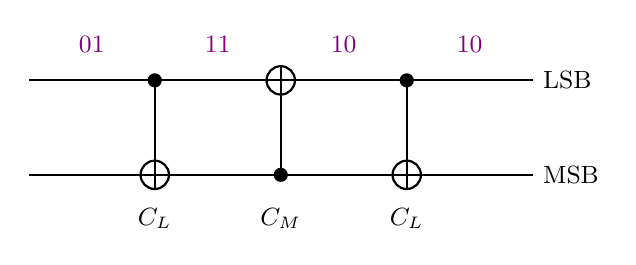
\begin{tikzpicture}[thick]
			% wires, LSB on top as in Figure 2
			\draw (0, 1.2) -- (6.4, 1.2) node[right] {\small LSB};
			\draw (0, 0) -- (6.4, 0) node[right] {\small MSB};

			% gate 1: LSB controls, MSB is the target
			\draw (1.6, 1.2) -- (1.6, 0);
			\fill (1.6, 1.2) circle (0.09);
			\draw (1.6, 0) circle (0.18);
			\draw (1.42, 0) -- (1.78, 0);
			\draw (1.6, -0.18) -- (1.6, 0.18);

			% gate 2: MSB controls, LSB is the target
			\draw (3.2, 0) -- (3.2, 1.2);
			\fill (3.2, 0) circle (0.09);
			\draw (3.2, 1.2) circle (0.18);
			\draw (3.02, 1.2) -- (3.38, 1.2);
			\draw (3.2, 1.02) -- (3.2, 1.38);

			% gate 3: LSB controls again
			\draw (4.8, 1.2) -- (4.8, 0);
			\fill (4.8, 1.2) circle (0.09);
			\draw (4.8, 0) circle (0.18);
			\draw (4.62, 0) -- (4.98, 0);
			\draw (4.8, -0.18) -- (4.8, 0.18);

			% example basis state |MSB LSB> between the gates
			\node[violet] at (0.8, 1.65) {\small \( \ket{01} \)};
			\node[violet] at (2.4, 1.65) {\small \( \ket{11} \)};
			\node[violet] at (4.0, 1.65) {\small \( \ket{10} \)};
			\node[violet] at (5.6, 1.65) {\small \( \ket{10} \)};
			\node at (1.6, -0.55) {\small \( C_L \)};
			\node at (3.2, -0.55) {\small \( C_M \)};
			\node at (4.8, -0.55) {\small \( C_L \)};
		\end{tikzpicture}
	\end{center}

	\noindent \textbf{Intuition method: following the bits.} Each CNOT XORs its control bit into its target bit, so for a basis state \( \ket{a\,b} \)
	\begin{align*}
		\ket{a\,b}
		 & \xrightarrow{\;C_L\;} \ket{a \oplus b,\; b}                                             \\
		 & \xrightarrow{\;C_M\;} \ket{a \oplus b,\; b \oplus (a \oplus b)} = \ket{a \oplus b,\; a} \\
		 & \xrightarrow{\;C_L\;} \ket{(a \oplus b) \oplus a,\; a} = \ket{b\,a},
	\end{align*}
	using \( x \oplus x = 0 \). The two bits end up exchanged. The example on top of the circuit is the case \( (a, b) = (0, 1) \): \( \ket{01} \to \ket{11} \to \ket{10} \to \ket{10} \).

	\noindent \textbf{Intuition method: following the amplitudes.} Every gate is linear, so it is enough to know which basis states it exchanges: \( C_L \) swaps \( \ket{01} \leftrightarrow \ket{11} \) and \( C_M \) swaps \( \ket{10} \leftrightarrow \ket{11} \).
	Starting from \( \ket{\Psi} = \alpha\ket{00} + \beta\ket{01} + \gamma\ket{10} + \delta\ket{11} \),
	\begin{align*}
		\ket{\Phi_1} = C_L\ket{\Psi}   & = \alpha\ket{00} + \delta\ket{01} + \gamma\ket{10} + \beta\ket{11}, \\
		\ket{\Phi_2} = C_M\ket{\Phi_1} & = \alpha\ket{00} + \delta\ket{01} + \beta\ket{10} + \gamma\ket{11}, \\
		\ket{\Phi} = C_L\ket{\Phi_2}   & = \alpha\ket{00} + \gamma\ket{01} + \beta\ket{10} + \delta\ket{11},
	\end{align*}
	so \( \beta \) and \( \gamma \) trade places while \( \alpha \) and \( \delta \) stay put: \( \ket{\Phi} = U_{\text{SWAP}}\ket{\Psi} \).

	\noindent \textbf{Matrix multiplication.} The circuit's matrix is now \( U' = C_L C_M C_L \). The first two gates give
	\[
		C_M C_L
		= \begin{pmatrix}
			1 & 0 & 0 & 0 \\ 0 & 1 & 0 & 0 \\ 0 & 0 & 0 & 1 \\ 0 & 0 & 1 & 0
		\end{pmatrix}
		\begin{pmatrix}
			1 & 0 & 0 & 0 \\ 0 & 0 & 0 & 1 \\ 0 & 0 & 1 & 0 \\ 0 & 1 & 0 & 0
		\end{pmatrix}
		= \begin{pmatrix}
			1 & 0 & 0 & 0 \\ 0 & 0 & 0 & 1 \\ 0 & 1 & 0 & 0 \\ 0 & 0 & 1 & 0
		\end{pmatrix},
	\]
	and the last \( C_L \), multiplied on the left, exchanges rows 2 and 4 (the rows of \( \ket{01} \) and \( \ket{11} \)):
	\[
		U' = C_L\paren{C_M C_L}
		= \begin{pmatrix}
			1 & 0 & 0 & 0 \\ 0 & 0 & 0 & 1 \\ 0 & 0 & 1 & 0 \\ 0 & 1 & 0 & 0
		\end{pmatrix}
		\begin{pmatrix}
			1 & 0 & 0 & 0 \\ 0 & 0 & 0 & 1 \\ 0 & 1 & 0 & 0 \\ 0 & 0 & 1 & 0
		\end{pmatrix}
		= \begin{pmatrix}
			1 & 0 & 0 & 0 \\ 0 & 0 & 1 & 0 \\ 0 & 1 & 0 & 0 \\ 0 & 0 & 0 & 1
		\end{pmatrix}
		= U_{\text{SWAP}} . \qquad \blacksquare
	\]

	\begin{remark}
		Both orderings work because SWAP is symmetric in the two qubits.
		Relabelling MSB \( \leftrightarrow \) LSB turns \( C_M \) into \( C_L \) and vice versa (\( C_L = U_{\text{SWAP}}\, C_M \,U_{\text{SWAP}} \), see \textbf{Problem 9}), so this circuit is the circuit of \textbf{Problem 3} drawn upside down -- and a gate that exchanges the two qubits cannot tell which way up it is drawn.
	\end{remark}
	The notebook (\textbf{Appendix~1}) confirms \( C_L C_M C_L = U_{\text{SWAP}} \) and traces all four basis states through the circuit.
\end{solution}
% ================================================================================ %

% ================================================================================ %
%                                    Problem 09                                    %
% ================================================================================ %
\begin{problem}
\textbf{LSB-Controlling CNOT Gate}
\par Repeat the definition and derivation of the CNOT gate matrix in \textbf{Chap.14} to obtain the matrix of LSB-controlling CNOT gate.
That is to derive \( U_{\text{XOR}, \text{center}}\) in the following equation:
\begin{align*}
	U_{\text{XOR}, \text{right}} U_{\text{XOR}, \text{center}} U_{\text{XOR}, \text{left}}
	 & = \begin{pmatrix}
		     1 & 0 & 0 & 0 \\
		     0 & 1 & 0 & 0 \\
		     0 & 0 & 0 & 1 \\
		     0 & 0 & 1 & 0
	     \end{pmatrix} \begin{pmatrix}
		                   1 & 0 & 0 & 0 \\
		                   0 & 0 & 0 & 1 \\
		                   0 & 0 & 1 & 0 \\
		                   0 & 1 & 0 & 0
	                   \end{pmatrix} \begin{pmatrix}
		                                 1 & 0 & 0 & 0 \\
		                                 0 & 1 & 0 & 0 \\
		                                 0 & 0 & 0 & 1 \\
		                                 0 & 0 & 1 & 0
	                                 \end{pmatrix} \\
	 & = \begin{pmatrix}
		     1 & 0 & 0 & 0 \\
		     0 & 0 & 0 & 1 \\
		     0 & 1 & 0 & 0 \\
		     0 & 0 & 1 & 0
	     \end{pmatrix} \begin{pmatrix}
		                   1 & 0 & 0 & 0 \\
		                   0 & 0 & 0 & 1 \\
		                   0 & 0 & 1 & 0 \\
		                   0 & 1 & 0 & 0
	                   \end{pmatrix}               \\
	 & = \begin{pmatrix}
		     1 & 0 & 0 & 0 \\
		     0 & 0 & 1 & 0 \\
		     0 & 1 & 0 & 0 \\
		     0 & 0 & 0 & 1
	     \end{pmatrix}                             \\
	U_{\text{XOR}, \text{right}} U_{\text{XOR}, \text{center}} U_{\text{XOR}, \text{left}}
	 & = U_{\text{SWAP}}
\end{align*}
\end{problem}

\begin{solution}
	\noindent \textbf{Definition.} A CNOT (XOR) gate writes the XOR of its control and target bits into the target and leaves the control unchanged.
	For the LSB-controlling gate the LSB \( b \) is the control and the MSB \( a \) is the target, so on \( \ket{a\,b} \)
	\[
		U_{\text{XOR},\text{center}}\ket{a\,b} = \ket{a \oplus b,\; b}.
	\]

	\noindent \textbf{Truth table.}
	\begin{center}
		\begin{tabular}{cccc}
			\toprule
			input \( \ket{a\,b} \) & control \( b \) & new MSB \( a \oplus b \) & output \( \ket{a \oplus b,\; b} \) \\
			\midrule
			\( \ket{00} \)         & \( 0 \)         & \( 0 \)                  & \( \ket{00} \)                     \\
			\( \ket{01} \)         & \( 1 \)         & \( 1 \)                  & \( \ket{11} \)                     \\
			\( \ket{10} \)         & \( 0 \)         & \( 1 \)                  & \( \ket{10} \)                     \\
			\( \ket{11} \)         & \( 1 \)         & \( 0 \)                  & \( \ket{01} \)                     \\
			\bottomrule
		\end{tabular}
	\end{center}

	\noindent \textbf{Building the matrix.} A gate that sends each basis input \( \ket{j} \) to a basis output \( \ket{f(j)} \) is \( U = \sum_j \ket{f(j)}\bra{j} \); indeed \( U\ket{k} = \sum_j \ket{f(j)}\braket{j \vert k} = \ket{f(k)} \).
	Reading the truth table row by row,
	\[
		U_{\text{XOR},\text{center}}
		= \ket{00}\bra{00} + \ket{11}\bra{01} + \ket{10}\bra{10} + \ket{01}\bra{11}.
	\]
	Each outer product \( \ket{i}\bra{j} \) is the matrix with a single \( 1 \) in row \( i \), column \( j \) (rows and columns ordered \( 00, 01, 10, 11 \)), so the four \( 1 \)s sit at \( (00, 00) \), \( (11, 01) \), \( (10, 10) \), and \( (01, 11) \):
	\[
		U_{\text{XOR},\text{center}}
		= \begin{pmatrix}
			1 & 0 & 0 & 0 \\
			0 & 0 & 0 & 1 \\
			0 & 0 & 1 & 0 \\
			0 & 1 & 0 & 0
		\end{pmatrix},
	\]
	the middle matrix of the equation, and the same \( C_L \) found column by column in \textbf{Problem 3}.

	\noindent \textbf{Compact form and a cross-check.} Grouping the terms by the value of the control (the LSB),
	\[
		U_{\text{XOR},\text{center}} = I \otimes \ket{0}\bra{0} + X \otimes \ket{1}\bra{1},
		\qquad\text{vs.}\qquad
		U_{\text{XOR},\text{left}} = U_{\text{XOR},\text{right}} = \ket{0}\bra{0} \otimes I + \ket{1}\bra{1} \otimes X,
	\]
	the mirror image of the MSB-controlling gate. Mirroring the two qubits is exactly what SWAP does, and indeed
	\[
		U_{\text{SWAP}}\, U_{\text{XOR},\text{left}}\, U_{\text{SWAP}} :
		\ket{a\,b} \mapsto \ket{b\,a} \mapsto \ket{b,\; b \oplus a} \mapsto \ket{a \oplus b,\; b}
		= U_{\text{XOR},\text{center}}\ket{a\,b}.
	\]

	\noindent \textbf{The full equation.} \( U_{\text{XOR},\text{left}} = U_{\text{XOR},\text{right}} \) swaps \( \ket{10} \leftrightarrow \ket{11} \), so multiplying by it on the left exchanges rows 3 and 4 and multiplying on the right exchanges columns 3 and 4:
	\begin{align*}
		U_{\text{XOR},\text{right}}\, U_{\text{XOR},\text{center}}
		 & = \begin{pmatrix}
			     1 & 0 & 0 & 0 \\ 0 & 0 & 0 & 1 \\ 0 & 1 & 0 & 0 \\ 0 & 0 & 1 & 0
		     \end{pmatrix}
		\quad (\text{rows 3, 4 of } U_{\text{XOR},\text{center}} \text{ exchanged}), \\
		\paren{U_{\text{XOR},\text{right}}\, U_{\text{XOR},\text{center}}}\, U_{\text{XOR},\text{left}}
		 & = \begin{pmatrix}
			     1 & 0 & 0 & 0 \\ 0 & 0 & 1 & 0 \\ 0 & 1 & 0 & 0 \\ 0 & 0 & 0 & 1
		     \end{pmatrix}
		= U_{\text{SWAP}}
		\quad (\text{columns 3, 4 exchanged}),
	\end{align*}
	reproducing every line of the given equation. \( \blacksquare \)
	The notebook (\textbf{Appendix~1}) builds \( U_{\text{XOR},\text{center}} \) from the outer-product sum and checks it against both closed forms and the full product.
\end{solution}
% ================================================================================ %

\newpage

% ================================================================================ %
%                                    Problem 10                                    %
% ================================================================================ %
\begin{problem}
\textbf{Quantum Computing Exercise 1}
\par Run the basis transformation circuit in \textbf{Figure 1} on IBM-Q using real hardware and simulation.
Do necessary modification to change the input to \( \ket{11} \) and check the output.
\fig[0.6\linewidth]{images/problem-10-1.png}{The Quantum Circuit}{quantum-circuit}
\fig[0.6\linewidth]{images/problem-10-2.png}{Implementation of a SWAP gate using CNOT gates.
	The purple ket's on top shows an example of how a single basis vector evolves in the circuit.}{SWAP-from-CNOT}
\end{problem}

\begin{solution}
	\noindent \textbf{What the circuit does.} In \textbf{Figure 1} the MSB \( q_1 \) gets a Hadamard and then controls a CNOT onto \( q_0 \); the \( I \) on \( q_0 \) is an identity placeholder.
	For an input \( \ket{a\,b} \) (MSB first),
	\begin{align*}
		\ket{a\,b}
		 & \xrightarrow{\;H \otimes I\;} \tfrac{1}{\sqrt{2}}\paren{\ket{0} + (-1)^{a}\ket{1}} \otimes \ket{b}       \\
		 & \xrightarrow{\;\mathrm{CNOT}\;} \tfrac{1}{\sqrt{2}}\paren{\ket{0,\, b} + (-1)^{a}\ket{1,\, 1 \oplus b}},
	\end{align*}
	so the circuit maps the computational basis onto the four Bell states -- hence ``basis transformation'':
	\begin{center}
		\begin{tabular}{ccc}
			\toprule
			input          & output                                                                & measured bit strings                 \\
			\midrule
			\( \ket{00} \) & \( \ket{\phi^{+}} = \tfrac{1}{\sqrt{2}}\paren{\ket{00} + \ket{11}} \) & \texttt{00}, \texttt{11} (50\% each) \\
			\( \ket{01} \) & \( \ket{\psi^{+}} = \tfrac{1}{\sqrt{2}}\paren{\ket{01} + \ket{10}} \) & \texttt{01}, \texttt{10} (50\% each) \\
			\( \ket{10} \) & \( \ket{\phi^{-}} = \tfrac{1}{\sqrt{2}}\paren{\ket{00} - \ket{11}} \) & \texttt{00}, \texttt{11} (50\% each) \\
			\( \ket{11} \) & \( \ket{\psi^{-}} = \tfrac{1}{\sqrt{2}}\paren{\ket{01} - \ket{10}} \) & \texttt{01}, \texttt{10} (50\% each) \\
			\bottomrule
		\end{tabular}
	\end{center}
	Run as given, the composer starts from \( \ket{00} \), so both the simulator and the hardware should show two bars, \texttt{00} and \texttt{11}, at about 50\% each.

	\noindent \textbf{Changing the input to \( \ket{11} \).} The composer always starts in \( \ket{00} \), so \( \ket{11} \) has to be prepared with a NOT on each qubit: replace the \( I \) on \( q_0 \) with \( X \), and put an \( X \) before the \( H \) on \( q_1 \).

	\begin{center}
		\begin{tikzpicture}[>=Stealth, thick]
			% wires -- bottom qubit is the MSB in IBM-Q
			\draw (0, 1.2) -- (5.8, 1.2);
			\draw (0, 0) -- (5.8, 0);
			\node[left] at (0, 1.2) {\small \( q_0 \) (LSB): \( \ket{0} \)};
			\node[left] at (0, 0) {\small \( q_1 \) (MSB): \( \ket{0} \)};

			% input preparation |00> -> |11>
			\draw[dashed, gray] (0.35, -0.55) rectangle (1.35, 1.75);
			\node[gray, above] at (0.85, 1.75) {\footnotesize input \( \ket{11} \)};
			\draw[fill=white] (0.5, 0.85) rectangle (1.2, 1.55);
			\node at (0.85, 1.2) {\( X \)};
			\draw[fill=white] (0.5, -0.35) rectangle (1.2, 0.35);
			\node at (0.85, 0) {\( X \)};

			% Figure 1: H on the MSB, then CNOT (control MSB, target LSB)
			\draw[fill=white] (1.9, -0.35) rectangle (2.6, 0.35);
			\node at (2.25, 0) {\( H \)};
			\draw (3.5, 0) -- (3.5, 1.2);
			\fill (3.5, 0) circle (0.09);
			\draw (3.5, 1.2) circle (0.18);
			\draw (3.32, 1.2) -- (3.68, 1.2);
			\draw (3.5, 1.02) -- (3.5, 1.38);

			% measurements
			\draw[fill=white] (4.6, 0.85) rectangle (5.3, 1.55);
			\draw (4.75, 1.05) arc (180:0:0.2);
			\draw[->] (4.95, 1.05) -- (5.12, 1.4);
			\draw[fill=white] (4.6, -0.35) rectangle (5.3, 0.35);
			\draw (4.75, -0.15) arc (180:0:0.2);
			\draw[->] (4.95, -0.15) -- (5.12, 0.2);
		\end{tikzpicture}
	\end{center}

	\noindent \textbf{Expected output.} Step by step, MSB first,
	\begin{align*}
		\paren{X \otimes X}\ket{00}                                   & = \ket{11},                                                                                                      \\
		\paren{H \otimes I}\ket{11}                                   & = \tfrac{1}{\sqrt{2}}\paren{\ket{0} - \ket{1}} \otimes \ket{1} = \tfrac{1}{\sqrt{2}}\paren{\ket{01} - \ket{11}}, \\
		\mathrm{CNOT}\,\tfrac{1}{\sqrt{2}}\paren{\ket{01} - \ket{11}} & = \tfrac{1}{\sqrt{2}}\paren{\ket{01} - \ket{10}} = \ket{\psi^{-}},
	\end{align*}
	so \( \mathrm{P}(\texttt{01}) = \mathrm{P}(\texttt{10}) = \tfrac{1}{2} \) and \( \mathrm{P}(\texttt{00}) = \mathrm{P}(\texttt{11}) = 0 \).

	\noindent \textbf{Running it.} Both versions were built in Qiskit exactly as drawn and run with 1024 shots each on the ideal \texttt{AerSimulator} and on the IBM processor \texttt{ibm\_marrakesh} (job \texttt{dar2ndrt55cs738sgol0}, physical qubits 153 and 154):
	\begin{codingbox*}
qc = QuantumCircuit(2, 2)
qc.x([0, 1])                  # input |11>   (Figure 1 as given: qc.id(0) instead)
qc.h(1)                       # H on the MSB
qc.cx(1, 0)                   # CNOT, MSB controls
qc.measure([0, 1], [0, 1])    # bit string c1 c0, as in the composer
\end{codingbox*}
	\begin{center}
		\begin{tabular}{lcccc}
			\toprule
			counts (1024 shots)                           & \texttt{00} & \texttt{01} & \texttt{10} & \texttt{11} \\
			\midrule
			input \( \ket{00} \), simulator               & 521         & 0           & 0           & 503         \\
			input \( \ket{00} \), \texttt{ibm\_marrakesh} & 519         & 5           & 10          & 490         \\
			input \( \ket{11} \), simulator               & 0           & 503         & 521         & 0           \\
			input \( \ket{11} \), \texttt{ibm\_marrakesh} & 15          & 498         & 506         & 5           \\
			\bottomrule
		\end{tabular}
	\end{center}
	\fig*[0.85\linewidth]{images/problem-10-answer.png}{}{}
	\noindent Both runs match the prediction. The simulator splits each Bell state between its two strings within the expected statistical fluctuation of \( \sqrt{1024 \cdot \tfrac{1}{2} \cdot \tfrac{1}{2}} = 16 \) shots.
	On the hardware, 98.5\% (input \( \ket{00} \)) and 98.0\% (input \( \ket{11} \)) of the shots land on the two correct strings; the remaining 1.5--2\% are gate and readout errors.
	The modified circuit therefore outputs \texttt{01}/\texttt{10} at 50\% each, i.e.\ \( \ket{\psi^{-}} \) -- up to its minus sign, which a histogram cannot see (see the remark below).
	The full code and output are in the notebook (\textbf{Appendix~1}).

	\begin{remark}[A first attempt that went wrong]
		The same five circuits of Problems 10--12 were first run on \texttt{ibm\_kingston} with the default qubit choice, physical qubits 0 and 1 (job \texttt{dar2lobt55cs738sgmo0}).
		Only 67\% and 57\% of the shots landed on the correct strings here, and 50\%, 38\%, and 40\% in Problems 11 and 12 -- even though the exact circuits the device received simulate perfectly, and that pair's published calibration (CZ error 0.08\%, readout error 1--2\%) promised far better.
		Calibration data are snapshots taken hours earlier, and a qubit pair can drift in between.
		Re-running on the best-calibrated pair of \texttt{ibm\_marrakesh} gave the clean results reported here. On real hardware, \emph{which} physical qubits run the circuit matters as much as the circuit itself.
	\end{remark}

	\begin{remark}
		A computational-basis histogram cannot see the minus sign: \( \ket{\psi^{+}} \) (input \( \ket{01} \)) gives exactly the same two bars as \( \ket{\psi^{-}} \).
		To confirm the output really is \( \ket{\psi^{-}} \), undo the transformation before measuring (a CNOT and then \( H \) on \( q_1 \)), which returns \( \ket{11} \) with certainty.
	\end{remark}
\end{solution}
% ================================================================================ %

% ================================================================================ %
%                                    Problem 11                                    %
% ================================================================================ %
\begin{problem}
\textbf{Quantum Computing Exercise 2}
\par Run the SWAP circuit in \textbf{Figure 2}, on IBM-Q using real hardware and simulation.
Do necessary modification to change the input to \( \ket{10} \) and check the output.
\end{problem}

\begin{solution}
	\noindent \textbf{Setting up the input.} \textbf{Figure 3} shows the SWAP circuit of \textbf{Figure 2} built in IBM-Q: a NOT on \( q_0 \) prepares \( \ket{q_1 q_0} = \ket{01} \), followed by CNOTs controlled by \( q_1 \), \( q_0 \), \( q_1 \) -- that is, \( C_M \), \( C_L \), \( C_M \) of \textbf{Problem 3}.
	To feed in \( \ket{10} \) instead, move the NOT gate from \( q_0 \) to \( q_1 \), the MSB:

	\begin{center}
		\begin{tikzpicture}[>=Stealth, thick]
			% wires -- bottom qubit is the MSB in IBM-Q
			\draw (0, 1.2) -- (5.9, 1.2);
			\draw (0, 0) -- (5.9, 0);
			\node[left] at (0, 1.2) {\small \( q_0 \) (LSB): \( \ket{0} \)};
			\node[left] at (0, 0) {\small \( q_1 \) (MSB): \( \ket{0} \)};

			% input preparation |00> -> |10>
			\draw[fill=white] (0.5, -0.35) rectangle (1.2, 0.35);
			\node at (0.85, 0) {\( X \)};

			% C_M: control q1, target q0
			\draw (2.0, 0) -- (2.0, 1.2);
			\fill (2.0, 0) circle (0.09);
			\draw (2.0, 1.2) circle (0.18);
			\draw (1.82, 1.2) -- (2.18, 1.2);
			\draw (2.0, 1.02) -- (2.0, 1.38);

			% C_L: control q0, target q1
			\draw (3.0, 1.2) -- (3.0, 0);
			\fill (3.0, 1.2) circle (0.09);
			\draw (3.0, 0) circle (0.18);
			\draw (2.82, 0) -- (3.18, 0);
			\draw (3.0, -0.18) -- (3.0, 0.18);

			% C_M again
			\draw (4.0, 0) -- (4.0, 1.2);
			\fill (4.0, 0) circle (0.09);
			\draw (4.0, 1.2) circle (0.18);
			\draw (3.82, 1.2) -- (4.18, 1.2);
			\draw (4.0, 1.02) -- (4.0, 1.38);

			% measurements
			\draw[fill=white] (4.8, 0.85) rectangle (5.5, 1.55);
			\draw (4.95, 1.05) arc (180:0:0.2);
			\draw[->] (5.15, 1.05) -- (5.32, 1.4);
			\draw[fill=white] (4.8, -0.35) rectangle (5.5, 0.35);
			\draw (4.95, -0.15) arc (180:0:0.2);
			\draw[->] (5.15, -0.15) -- (5.32, 0.2);
		\end{tikzpicture}
	\end{center}

	\noindent \textbf{Expected output.} Following the bits \( (a, b) = (1, 0) \) (MSB first):
	\[
		\ket{10}
		\xrightarrow{\;C_M\;} \ket{1,\; 1 \oplus 0} = \ket{11}
		\xrightarrow{\;C_L\;} \ket{1 \oplus 1,\; 1} = \ket{01}
		\xrightarrow{\;C_M\;} \ket{0,\; 0 \oplus 1} = \ket{01},
	\]
	so the output is \( U_{\text{SWAP}}\ket{10} = \ket{01} \). It is a basis state, so it is measured with certainty: \( \mathrm{P}(\texttt{01}) = 100\% \), read in the composer's \( c_1 c_0 \) bit string as \texttt{01}.

	\noindent \textbf{Running it.} Run with 1024 shots on the \texttt{AerSimulator} and on \texttt{ibm\_marrakesh} (same job and qubits as \textbf{Problem 10}):
	\begin{center}
		\begin{tabular}{lcccc}
			\toprule
			counts (1024 shots)     & \texttt{00} & \texttt{01} & \texttt{10} & \texttt{11} \\
			\midrule
			simulator               & 0           & 1024        & 0           & 0           \\
			\texttt{ibm\_marrakesh} & 19          & 989         & 9           & 7           \\
			\bottomrule
		\end{tabular}
	\end{center}
	\fig*[0.8\linewidth]{images/problem-11-answer.png}{}{}
	\noindent The simulator puts every shot on \texttt{01}, and the hardware puts 989 of 1024 (96.6\%) there -- the SWAP works as predicted.
	The largest error bar is \texttt{00} (19 shots): the \( \ket{1} \) that ends up in \( q_0 \) relaxing back to \( \ket{0} \), the same bias discussed in \textbf{Problem 12}.
	A handy sanity check is that the result mirrors \textbf{Figure 3}: there input \( \ket{01} \) gives \texttt{10}; here input \( \ket{10} \) gives \texttt{01}.
\end{solution}
% ================================================================================ %

% ================================================================================ %
%                                    Problem 12                                    %
% ================================================================================ %
\begin{problem}
\textbf{Quantum Computing Exercise 3}
\par Run the SWAP circuit in \textbf{Figure 2} on IBM-Q
using real hardware and simulation but use the SWAP gate directly instead of using CNOT gates.
Compare the outputs to \textbf{Figure 3}
\fig[0.6\linewidth]{images/problem-12.png}{The quantum circuit in \textbf{Figure 1} built in IBM-Q.
	The simulation result is shown in the middle,
	and the real quantum computer execution result is shown on the right.}{problem-12-result}
\end{problem}

\begin{solution}
	\noindent \textbf{The circuit.} Keep the input of \textbf{Figure 3} (a NOT on \( q_0 \), so \( \ket{q_1 q_0} = \ket{01} \)) and replace the three CNOTs with the composer's built-in SWAP gate:

	\begin{center}
		\begin{tikzpicture}[>=Stealth, thick]
			% wires -- bottom qubit is the MSB in IBM-Q
			\draw (0, 1.2) -- (4.2, 1.2);
			\draw (0, 0) -- (4.2, 0);
			\node[left] at (0, 1.2) {\small \( q_0 \) (LSB): \( \ket{0} \)};
			\node[left] at (0, 0) {\small \( q_1 \) (MSB): \( \ket{0} \)};

			% input preparation |00> -> |01>
			\draw[fill=white] (0.5, 0.85) rectangle (1.2, 1.55);
			\node at (0.85, 1.2) {\( X \)};

			% SWAP gate
			\draw (2.1, 0) -- (2.1, 1.2);
			\draw (1.95, 1.05) -- (2.25, 1.35);
			\draw (1.95, 1.35) -- (2.25, 1.05);
			\draw (1.95, -0.15) -- (2.25, 0.15);
			\draw (1.95, 0.15) -- (2.25, -0.15);

			% measurements
			\draw[fill=white] (3.1, 0.85) rectangle (3.8, 1.55);
			\draw (3.25, 1.05) arc (180:0:0.2);
			\draw[->] (3.45, 1.05) -- (3.62, 1.4);
			\draw[fill=white] (3.1, -0.35) rectangle (3.8, 0.35);
			\draw (3.25, -0.15) arc (180:0:0.2);
			\draw[->] (3.45, -0.15) -- (3.62, 0.2);
		\end{tikzpicture}
	\end{center}

	\noindent \textbf{Simulation: identical to Figure 3.} \textbf{Problem 3} proved \( C_M C_L C_M = U_{\text{SWAP}} \) as matrices, so the two circuits implement the same unitary and produce the same output state,
	\[
		U_{\text{SWAP}}\ket{01} = \ket{10} = C_M C_L C_M\ket{01},
	\]
	which is measured as \texttt{10} with probability 100\% -- the single bar of the simulation in \textbf{Figure 3}.
	The notebook (\textbf{Appendix~1}) runs both versions and finds identical state vectors.

	\noindent \textbf{Running it.} Both versions -- the three CNOTs of \textbf{Figure 3} and the direct SWAP gate -- were run side by side with 1024 shots each on the \texttt{AerSimulator} and on \texttt{ibm\_marrakesh} (same job and qubits as \textbf{Problem 10}):
	\begin{center}
		\begin{tabular}{lcccc}
			\toprule
			counts (1024 shots)                  & \texttt{00} & \texttt{01} & \texttt{10} & \texttt{11} \\
			\midrule
			three CNOTs, simulator               & 0           & 0           & 1024        & 0           \\
			three CNOTs, \texttt{ibm\_marrakesh} & 16          & 8           & 993         & 7           \\
			SWAP gate, simulator                 & 0           & 0           & 1024        & 0           \\
			SWAP gate, \texttt{ibm\_marrakesh}   & 18          & 10          & 986         & 10          \\
			\bottomrule
		\end{tabular}
	\end{center}
	\fig*[0.85\linewidth]{images/problem-12-answer.png}{}{}

	\noindent \textbf{Comparison with Figure 3.}
	\begin{itemize}
		\item \textbf{Simulation:} identical -- every shot on \texttt{10}, for both versions and in \textbf{Figure 3}.
		\item \textbf{Real hardware:} the SWAP gate puts 96.3\% of the shots on \texttt{10} and the three CNOTs 97.0\%. The 7-shot difference is within one standard deviation of shot noise (about 8 shots), so the two are statistically the same. Both beat the roughly 90\% of the textbook's hardware run in \textbf{Figure 3}.
		\item \textbf{Why they match:} IBM processors have no native SWAP. Transpiling for \texttt{ibm\_marrakesh} (optimization level 1, as used for the run) turns the SWAP gate into \emph{three} CZ gates -- exactly as many as the three-CNOT version -- so the device executes essentially the circuit of \textbf{Figure 3} either way.
	\end{itemize}
	At optimization level 3 the transpiler goes further and removes this SWAP entirely (0 CZ gates), because a SWAP right before measurement can be replaced by relabelling which qubit feeds which classical bit. The three-CNOT version still costs three CZ gates there, as the notebook (\textbf{Appendix~1}) shows.

	\begin{remark}
		The largest wrong outcome is \texttt{00} in both of our runs (16 and 18 shots) and in \textbf{Figure 3}: the correct result \texttt{10} with \( q_1 \) fallen back to \( \ket{0} \).
		That pattern is consistent with energy relaxation (\( T_1 \) decay, \( \ket{1} \to \ket{0} \)) during the gates and readout, the dominant error on superconducting qubits -- errors push outcomes toward \texttt{0}s, whichever way the SWAP is built.
	\end{remark}
\end{solution}
% ================================================================================ %

% ================================================================================ %
%                                     Appendix                                     %
% ================================================================================ %

\myappendix{code/assignment-07-code.pdf}{Assignment 07 | Code Solution}

% ================================================================================ %

\end{document}
